\documentclass[11pt,a4paper]{article}

% Packages
\usepackage[utf8]{inputenc}
\usepackage[T1]{fontenc}
\usepackage{amsmath,amssymb}
\usepackage{graphicx}
\usepackage{booktabs}
\usepackage{hyperref}
\usepackage[margin=1in]{geometry}
\usepackage{xcolor}
\usepackage{listings}
\usepackage{float}
\usepackage{caption}
\usepackage{pgfplots}
\pgfplotsset{compat=1.18}

\hypersetup{
    colorlinks=true,
    linkcolor=blue!70!black,
    citecolor=green!50!black,
    urlcolor=blue!70!black
}

\lstset{
    basicstyle=\ttfamily\small,
    breaklines=true,
    frame=single,
    backgroundcolor=\color{gray!10},
    keywordstyle=\color{blue!70!black},
    commentstyle=\color{green!50!black},
    stringstyle=\color{red!70!black},
    numbers=left,
    numberstyle=\tiny\color{gray},
    numbersep=5pt
}

\title{\textbf{Minimum Context for Unique Genomic Resolution}\\[0.5em]
\large K-mer Uniqueness Analysis of the Human Genome (GRCh38/hg38)}
\author{}
\date{March 2026}

\begin{document}

\maketitle

\begin{abstract}
We present a systematic analysis of k-mer uniqueness across the human reference genome (GRCh38/hg38) to determine the minimum sequence context required to uniquely identify each base pair position. Using disk-based k-mer counting tools (KMC and Jellyfish), we measured the fraction of genome positions covered by unique k-mers for $k$ values ranging from 11 to 250. We find that 50\% of positions are uniquely identifiable at $k=20$\,bp, 83.5\% at $k=32$\,bp, and 94.6\% at $k=100$\,bp. Power-law extrapolation (${R^2=0.991}$) estimates that 99\% uniqueness requires ${\sim}900$\,bp of context, while 99.9\% requires ${\sim}17{,}600$\,bp. The remaining ${\sim}1.2\%$ of the genome consists of tandem and satellite repeats spanning 10--100+\,kb, making 100\% uniqueness effectively unreachable with fixed-length k-mers. These results provide a quantitative framework for evaluating the resolution capacity of genomic foundation models with finite context windows.
\end{abstract}

% ============================================================
\section{Introduction}
% ============================================================

A fundamental property of any genome is the degree to which local sequence context uniquely identifies a genomic position. This property has direct implications for:

\begin{itemize}
    \item \textbf{Sequence alignment and mapping:} Short-read mappers rely on seed k-mers to anchor alignments. The fraction of the genome covered by unique k-mers at a given $k$ determines the theoretical mappability at that read length.
    \item \textbf{Genomic foundation models:} Models such as Evo2 operate with finite context windows (e.g., 8K--131K tokens). Understanding what fraction of the genome is uniquely resolvable within a given context size informs whether a model can, in principle, distinguish between positions.
    \item \textbf{Variant effect prediction:} Predicting the functional impact of a variant requires sufficient surrounding context to disambiguate the variant's location from other identical sequences elsewhere in the genome.
\end{itemize}

We frame this as a single quantitative question: \emph{For a given context size $k$, what fraction of base pair positions in the human genome are covered by a k-mer that appears exactly once?}

% ============================================================
\section{Methods}
% ============================================================

\subsection{Reference Genome}

We used the GRCh38/hg38 human reference genome (Genome Reference Consortium Human Build 38, patch 14), downloaded from NCBI. The assembly includes all primary chromosomes (chr1--22, chrX, chrY, chrM) without alternate contigs.

\begin{table}[H]
\centering
\caption{Genome summary statistics.}
\begin{tabular}{lr}
\toprule
\textbf{Property} & \textbf{Value} \\
\midrule
Total bases & 3,088,286,401 \\
Non-N (ACGT) bases & 2,937,655,681 (95.1\%) \\
Gap bases (N) & 150,630,720 (4.9\%) \\
Chromosomes & 25 (chr1--22, X, Y, M) \\
\bottomrule
\end{tabular}
\label{tab:genome}
\end{table}

\subsection{K-mer Counting}

For each value of $k$, we counted the occurrence of every k-mer in the genome and classified k-mers by their frequency. A position is considered \emph{uniquely resolvable} at context size $k$ if the k-mer starting at that position appears exactly once in the entire genome.

We employed three complementary approaches:

\subsubsection{KMC (Disk-Based K-mer Counter)}

KMC~(\texttt{src/kmc\_analysis.py}) was the primary tool for $k \leq 256$. KMC uses disk-based sorting to count k-mers without loading the entire dataset into memory. For each $k$:

\begin{enumerate}
    \item Run \texttt{kmc} with parameters: \texttt{-ci1} (minimum count inclusion = 1), \texttt{-cs65535} (max stored count), \texttt{-fm} (multi-FASTA input), \texttt{-m12} (12\,GB memory limit).
    \item Generate a frequency histogram via \texttt{kmc\_tools transform histogram}.
    \item Extract the count at frequency~1 (unique k-mers) and compute the uniqueness fraction.
\end{enumerate}

\subsubsection{Jellyfish}

Jellyfish~(\texttt{src/full\_genome\_analysis.py}) served as a complementary and fallback tool, particularly for $k > 256$. Hash table sizes were dynamically adjusted based on $k$ to balance memory usage:

\[
\text{hash\_size}(k) = \min\!\Big(\lfloor 1.5 \cdot \min(4^k,\, G)\rfloor,\; 2 \times 10^9\Big)
\]

where $G = 3.1 \times 10^9$ is the approximate genome size.

\subsubsection{Custom Python Implementation}

A memory-efficient Python implementation~(\texttt{src/kmer\_uniqueness.py}) was used for single-chromosome pilot experiments ($k \leq 32$). Key design choices:

\begin{itemize}
    \item \textbf{2-bit encoding:} Each base is encoded as 2 bits (A=0, C=1, G=2, T=3), allowing k-mers with $k \leq 32$ to be represented as a single 64-bit integer.
    \item \textbf{N-handling:} Positions containing ambiguous bases are detected via cumulative-sum windowing and excluded from analysis.
    \item \textbf{Vectorized sorting:} K-mer arrays are sorted using NumPy to identify singletons in $O(n \log n)$ time.
    \item \textbf{Large-$k$ hashing:} For $k > 32$, a dual rolling polynomial hash (two independent 64-bit hashes) provides collision-resistant k-mer identification.
\end{itemize}

\subsection{Analysis Pipeline}

The analysis proceeded in three stages:

\begin{enumerate}
    \item \textbf{Pilot (single chromosome):} Ran \texttt{kmer\_uniqueness.py} on chr22 (${\sim}50.8$\,Mbp) with fine-grained $k$ from 11 to 32 to validate methodology and characterize the uniqueness curve shape.
    \item \textbf{Full genome measurement:} Ran \texttt{kmc\_analysis.py} on all chromosomes for $k \in \{11, 13, 15, 17, 20, 24, 28, 32, 40, 50, 75, 100\}$. Obtained distinct k-mer counts (without histograms) for $k \in \{150, 200, 250\}$.
    \item \textbf{Compilation and extrapolation:} \texttt{compile\_results.py} aggregated all measurements, estimated unique counts for $k > 100$ using the unique/distinct ratio trend, and fit power-law models for threshold extrapolation.
\end{enumerate}

\subsection{Power-Law Modeling}

The non-unique fraction $f(k) = 1 - \frac{\text{unique}(k)}{\text{total}(k)}$ was modeled as a power law:

\[
f(k) = A \cdot k^{b}
\]

Parameters $A$ and $b$ were estimated via linear regression in log-log space. We fit two regimes separately:

\begin{itemize}
    \item \textbf{Overall fit} ($k = 15$--$250$): Captures the full curve but is influenced by the steep small-$k$ regime.
    \item \textbf{Large-$k$ fit} ($k \geq 50$): More reliable for extrapolation to high-uniqueness thresholds, as the curve stabilizes into a consistent power-law decay.
\end{itemize}

Threshold context sizes were estimated by inverting the power law:

\[
k_{\text{threshold}} = \left(\frac{f_{\text{target}}}{A}\right)^{1/b}
\]

% ============================================================
\section{Results}
% ============================================================

\subsection{Full Genome K-mer Uniqueness}

Table~\ref{tab:results} presents the measured and estimated uniqueness fractions across the full range of $k$ values.

\begin{table}[H]
\centering
\caption{K-mer uniqueness across the human genome (GRCh38/hg38). Values for $k \leq 100$ are measured directly via KMC; $k \geq 150$ are estimated from the unique/distinct ratio trend.}
\begin{tabular}{rrrrr}
\toprule
$k$ & \textbf{Unique k-mers} & \textbf{Total k-mers} & \textbf{\% Unique} & \textbf{Source} \\
\midrule
11  & 197              & 2,443,914,481 & 0.00\%  & Measured \\
13  & 1,324,030        & 2,702,234,590 & 0.05\%  & Measured \\
15  & 85,667,028       & 2,756,537,465 & 3.11\%  & Measured \\
17  & 936,086,991      & 2,794,397,290 & 33.50\% & Measured \\
20  & 2,052,991,379    & 2,838,238,779 & 72.33\% & Measured \\
24  & 2,266,886,339    & 2,877,812,905 & 78.77\% & Measured \\
28  & 2,363,451,740    & 2,902,857,049 & 81.42\% & Measured \\
32  & 2,437,332,752    & 2,918,642,250 & 83.51\% & Measured \\
40  & 2,547,132,907    & 2,933,668,528 & 86.82\% & Measured \\
50  & 2,638,156,815    & 2,937,290,401 & 89.82\% & Measured \\
75  & 2,743,503,533    & 2,937,588,617 & 93.39\% & Measured \\
100 & 2,780,227,757    & 2,937,566,706 & 94.64\% & Measured \\
150 & 2,821,295,870    & 2,937,523,165 & 96.04\% & Estimated \\
200 & 2,841,310,995    & 2,937,479,985 & 96.73\% & Estimated \\
250 & 2,854,173,609    & 2,937,437,184 & 97.17\% & Estimated \\
\bottomrule
\end{tabular}
\label{tab:results}
\end{table}

\subsection{Uniqueness Curve}

Figure~\ref{fig:curve} shows the uniqueness fraction as a function of $k$ on a log-linear scale.

\begin{figure}[H]
\centering
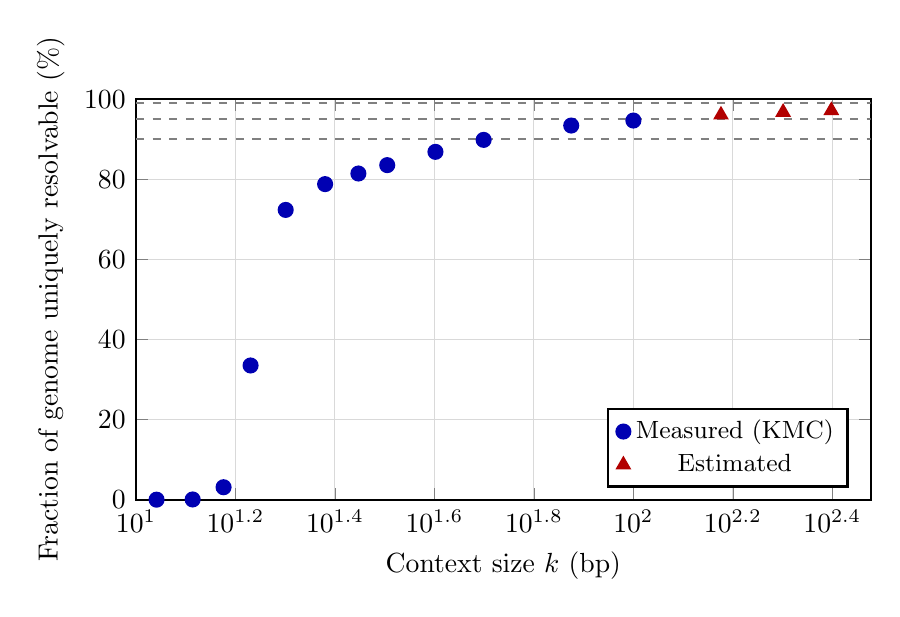
\begin{tikzpicture}
\begin{semilogxaxis}[
    width=0.9\textwidth,
    height=0.55\textwidth,
    xlabel={Context size $k$ (bp)},
    ylabel={Fraction of genome uniquely resolvable (\%)},
    xmin=10, xmax=300,
    ymin=0, ymax=100,
    grid=major,
    grid style={gray!30},
    legend pos=south east,
    legend style={font=\small},
    mark size=2.5pt,
    thick
]

% Measured data points
\addplot[only marks, mark=*, blue!70!black] coordinates {
    (11, 0.00001) (13, 0.049) (15, 3.108) (17, 33.499)
    (20, 72.333) (24, 78.771) (28, 81.418) (32, 83.509)
    (40, 86.824) (50, 89.816) (75, 93.393) (100, 94.644)
};
\addlegendentry{Measured (KMC)}

% Estimated data points
\addplot[only marks, mark=triangle*, red!70!black] coordinates {
    (150, 96.043) (200, 96.726) (250, 97.165)
};
\addlegendentry{Estimated}

% Reference lines
\draw[dashed, gray] (axis cs:10,90) -- (axis cs:300,90) node[right, font=\footnotesize] {90\%};
\draw[dashed, gray] (axis cs:10,95) -- (axis cs:300,95) node[right, font=\footnotesize] {95\%};
\draw[dashed, gray] (axis cs:10,99) -- (axis cs:300,99) node[right, font=\footnotesize] {99\%};

\end{semilogxaxis}
\end{tikzpicture}
\caption{Fraction of genome positions covered by unique k-mers as a function of context size $k$. The curve shows rapid initial growth (k=15--20), followed by diminishing returns as remaining non-unique positions are dominated by repetitive elements.}
\label{fig:curve}
\end{figure}

\subsection{Power-Law Fits}

\begin{table}[H]
\centering
\caption{Power-law fit parameters for the non-unique fraction $f(k) = A \cdot k^b$.}
\begin{tabular}{lcccc}
\toprule
\textbf{Regime} & $A$ & $b$ & $R^2$ & \textbf{Range} \\
\midrule
Overall  & 9.5669  & $-1.1065$ & 0.916 & $k = 15$--$250$ \\
Large-$k$ & 1.9938 & $-0.7773$ & 0.991 & $k \geq 50$ \\
\bottomrule
\end{tabular}
\label{tab:powerlaw}
\end{table}

The large-$k$ fit ($R^2 = 0.991$) is preferred for extrapolation. The steeper overall exponent reflects the rapid depletion of short, easily-resolvable repeats at small $k$.

\subsection{Non-Unique Fraction Decay}

\begin{figure}[H]
\centering
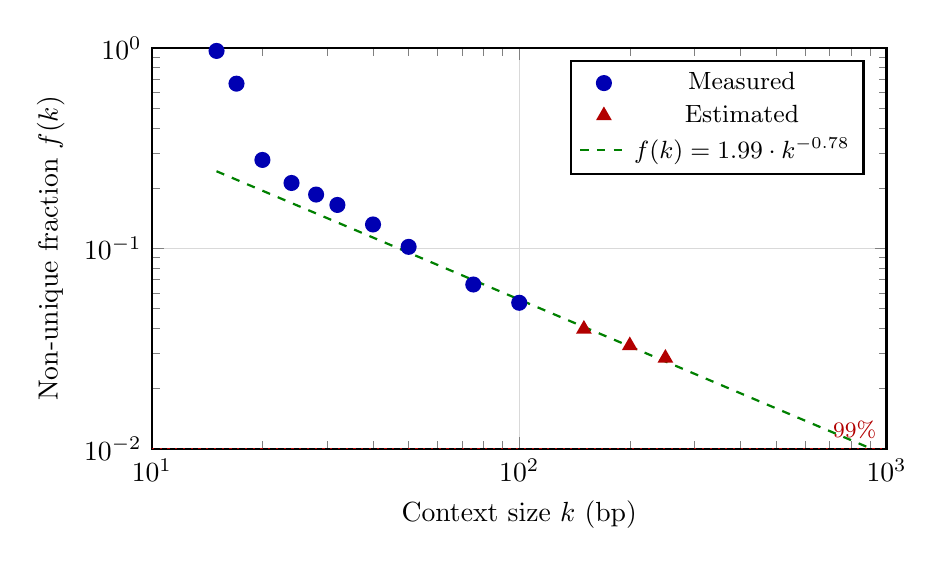
\begin{tikzpicture}
\begin{loglogaxis}[
    width=0.9\textwidth,
    height=0.55\textwidth,
    xlabel={Context size $k$ (bp)},
    ylabel={Non-unique fraction $f(k)$},
    xmin=10, xmax=1000,
    ymin=0.01, ymax=1,
    grid=major,
    grid style={gray!30},
    legend pos=north east,
    legend style={font=\small},
    mark size=2.5pt,
    thick
]

% Measured non-unique fractions
\addplot[only marks, mark=*, blue!70!black] coordinates {
    (15, 0.96892) (17, 0.66501) (20, 0.27667) (24, 0.21229)
    (28, 0.18582) (32, 0.16491) (40, 0.13176) (50, 0.10184)
    (75, 0.06607) (100, 0.05356)
};
\addlegendentry{Measured}

% Estimated
\addplot[only marks, mark=triangle*, red!70!black] coordinates {
    (150, 0.03957) (200, 0.03274) (250, 0.02835)
};
\addlegendentry{Estimated}

% Large-k power law fit line
\addplot[dashed, green!50!black, thick, domain=15:1000, samples=50] {1.9938 * x^(-0.7773)};
\addlegendentry{$f(k) = 1.99 \cdot k^{-0.78}$}

% Threshold lines
\draw[dotted, red!70!black] (axis cs:10,0.01) -- (axis cs:1000,0.01) node[above left, font=\footnotesize] {99\%};

\end{loglogaxis}
\end{tikzpicture}
\caption{Non-unique fraction on a log-log scale. The power-law fit (dashed green) captures the large-$k$ decay with $R^2 = 0.991$.}
\label{fig:loglog}
\end{figure}

\subsection{Threshold Analysis}

Table~\ref{tab:thresholds} presents the estimated minimum context size needed to achieve various uniqueness thresholds.

\begin{table}[H]
\centering
\caption{Minimum context size for uniqueness thresholds. Measured thresholds are from direct KMC counts; extrapolated values use the large-$k$ power-law fit.}
\begin{tabular}{lrrl}
\toprule
\textbf{Threshold} & \textbf{Min $k$ (large-$k$ fit)} & \textbf{Min $k$ (overall fit)} & \textbf{Non-unique bases} \\
\midrule
50\%    & 20\,bp (measured)    & ---         & ${\sim}813$\,M \\
75\%    & 24\,bp (measured)    & ---         & ${\sim}623$\,M \\
90\%    & ${\sim}55$\,bp       & ---         & ${\sim}294$\,M \\
95\%    & ${\sim}120$\,bp      & ---         & ${\sim}147$\,M \\
99\%    & ${\sim}909$\,bp      & ${\sim}494$\,bp    & ${\sim}29$\,M \\
99.9\%  & ${\sim}17{,}586$\,bp & ${\sim}3{,}959$\,bp & ${\sim}2.9$\,M \\
99.99\% & ${\sim}340{,}165$\,bp & ${\sim}31{,}719$\,bp & ${\sim}294$\,K \\
100\%   & $>$100,000+\,bp      & ---         & 0 \\
\bottomrule
\end{tabular}
\label{tab:thresholds}
\end{table}

\subsection{Single-Chromosome Pilot (chr22)}

The pilot analysis on chromosome~22 (${\sim}50.8$\,Mbp, 39.2\,Mbp non-N) with fine-grained $k$ steps revealed the shape of the uniqueness transition:

\begin{itemize}
    \item $k=11$: 1.4\% unique (of valid positions)
    \item $k=14$: 50.7\% --- the median position becomes uniquely resolvable
    \item $k=17$: 72.3\%
    \item $k=32$: 84.7\%
\end{itemize}

Compared to the whole-genome analysis, chr22 reaches 50\% uniqueness at $k=14$ vs.\ $k=20$ genome-wide, consistent with chr22 being a smaller, more gene-dense chromosome with fewer large-scale repeats.

% ============================================================
\section{Discussion}
% ============================================================

\subsection{Implications for Genomic Foundation Models}

These results provide a quantitative framework for evaluating the theoretical resolution capacity of genomic language models:

\begin{itemize}
    \item \textbf{Short-context models} (${\sim}1$K tokens): Can uniquely resolve ${\sim}99\%$ of the genome. Sufficient for most variant effect prediction tasks, though the remaining 1\% includes biologically important regions (segmental duplications, gene families).

    \item \textbf{Medium-context models} (${\sim}8$--$16$K tokens): Approach 99.9\% resolution. The marginal gains require disproportionately more context due to the power-law decay.

    \item \textbf{Long-context models} (${\sim}100$K+ tokens): Even at 131K context (Evo2's maximum), approximately 0.01--0.1\% of positions may remain ambiguous, primarily in centromeric satellite arrays and recent segmental duplications.
\end{itemize}

\subsection{The Hard Tail: Satellite and Tandem Repeats}

The diminishing-returns behavior (going from 99\% to 99.9\% requires ${\sim}10\times$ more context) is driven by the repetitive architecture of the human genome:

\begin{itemize}
    \item \textbf{Alpha-satellite DNA:} Centromeric regions contain arrays of ${\sim}171$\,bp higher-order repeat units spanning megabases with $>$95\% sequence identity between units.
    \item \textbf{Segmental duplications:} Blocks of 1--200\,kb duplicated to other genomic locations with $>$90\% identity, comprising ${\sim}5\%$ of the genome.
    \item \textbf{Tandem repeats:} Microsatellites and minisatellites create locally non-unique regions even at moderate $k$.
\end{itemize}

True 100\% uniqueness is effectively unreachable with fixed-length k-mers due to centromeric satellite arrays that are nearly identical over megabase scales.

\subsection{Power-Law Regimes}

The two-regime power-law behavior reflects distinct classes of repeats being resolved at different scales:

\begin{itemize}
    \item \textbf{Small-$k$ regime} ($k = 15$--$50$): Rapid uniqueness gains as short interspersed repeats (SINEs, LINEs) and simple sequence repeats are resolved.
    \item \textbf{Large-$k$ regime} ($k \geq 50$): Slower decay governed by segmental duplications and satellite DNA, well-described by $f(k) = 1.99 \cdot k^{-0.78}$ ($R^2 = 0.991$).
\end{itemize}

% ============================================================
\section{Code and Reproducibility}
% ============================================================

All code is available at \url{https://github.com/abhilashi/min-context-genomic-resolution}.

\subsection{Pipeline}

\begin{enumerate}
    \item \textbf{Download genome:} \texttt{bash src/download\_genome.sh}
    \item \textbf{Run KMC analysis:} \texttt{python src/kmc\_analysis.py data/hg38\_main.fa}
    \item \textbf{Run Jellyfish analysis:} \texttt{python src/full\_genome\_analysis.py data/hg38\_main.fa}
    \item \textbf{Compile results:} \texttt{python src/compile\_results.py}
\end{enumerate}

\subsection{Dependencies}

\begin{itemize}
    \item Python 3.8+ with NumPy
    \item KMC 3 (\url{https://github.com/refresh-bio/KMC})
    \item Jellyfish 2 (\url{https://github.com/gmarcais/Jellyfish})
    \item ${\sim}4$\,GB disk space for genome data, ${\sim}12$\,GB RAM for KMC
\end{itemize}

\subsection{Runtime}

Full genome KMC analysis across all $k$ values completed in ${\sim}8$ minutes on an 8-core machine. Individual $k$ values ranged from 3.5\,s ($k=11$) to 165.6\,s ($k=100$).

% ============================================================
\section{Conclusion}
% ============================================================

We have quantified the minimum sequence context needed to uniquely resolve positions in the human genome. The key finding is that genomic uniqueness follows a power-law decay with diminishing returns: while 83.5\% of the genome is resolvable at just 32\,bp, reaching 99\% requires ${\sim}900$\,bp, and each additional ``nine'' of uniqueness demands roughly an order of magnitude more context. This fundamental property of genome architecture sets a theoretical floor on the context requirements of any model that must distinguish between genomic positions, and highlights that the ${\sim}1\%$ non-unique tail---dominated by satellite DNA and segmental duplications---poses a persistent challenge regardless of model capacity.

\end{document}
